\keepTogether{
	\subsection{Befehlsformat}
	Geben Sie ein Befehlsformat für Assembler Befehle an. Beschriften sie die Blöcke mit ihrer Bitgröße:
	\begin{center}
		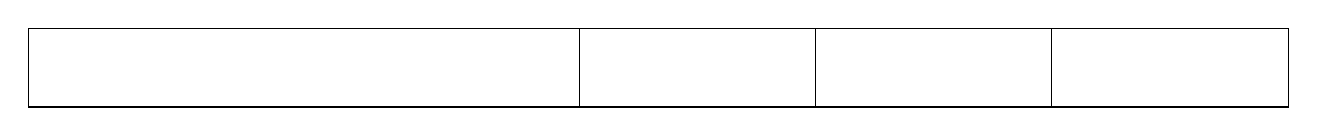
\begin{tikzpicture}
		\draw (0,0) rectangle (16,1);
		\draw (0,0) rectangle (7,1);
		\draw (7,0) rectangle (10,1);
		\draw (10,0) rectangle (13,1);
		\draw (13,0) rectangle (16,1);
		\end{tikzpicture}
	\end{center}
}\\[0.3cm]
%Aufgabe kommt hier her

%------------------------------------------------------------------------------------------------------------
%Befehle:
	
%Antwortboxen können folgendermaßen erzeugt werden:
%\makeanswerbox{height}
%\makeinlineanswrebox{length}{rechtes padding}
%\makecustomanswerbox{width}{height}

%Um Zeilenumbrüche innerhalb einer Aufgabe zu vermeiden nutze:
%\keepTogether{text}

%\subsubsection{} kann benutzt werden um die Aufgabe weiterhin zu unterteilen

%Falls deine Aufgabe zusätzliche usepackages benötigen sollte: trage sie einfach in die usepackage Datei in 
%ETIPAVorschlaege\SetupData\usepackage.tex ein schreibe die Funktion hinzu. packages die nicht annotiert sind,
%werden nicht akzeptiert